\begin{center}
    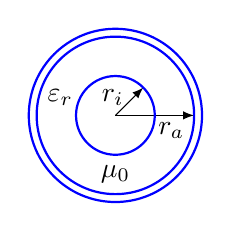
\begin{tikzpicture}
        \draw[-latex](0,0) --(1,0);
        \node at (-0.7,0)[above]{$\varepsilon_r$};
        \node at (1,0)[below left, yshift=1pt]{$ r_a $};
        \draw[-latex, rotate=45](0,0)--(.5,0);
        \node at (0,0)[above, xshift=-1pt]{$ r_i $};
        \draw[-, thick, blue](0,0) circle (1);
        \draw[-, thick, blue](0,0) circle (1.10);
        \node at(0,-.75)[]{$\mu_0$};
        \draw[-, thick, blue](0,0) circle (0.5);
        
    \end{tikzpicture}


%    D = Außendurchmesser

%    d = Innendurchmesser
\end{center}
\vspace{-1em}
